% Editable source for radar.pdf. Build with: pdflatex radar.tex
\documentclass[tikz,border=5pt]{standalone}
\usepackage[T1]{fontenc}
\usepackage{lmodern}
\begin{document}
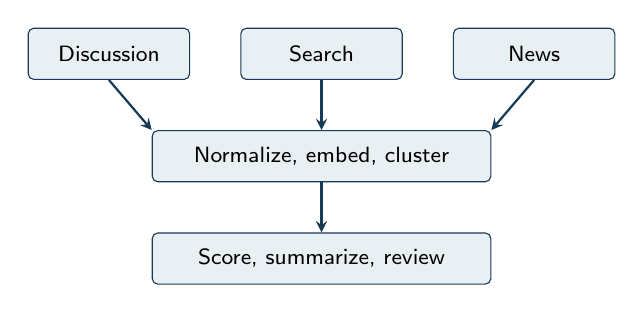
\begin{tikzpicture}[font=\sffamily\footnotesize,>=stealth]
  \definecolor{ink}{HTML}{173A56}
  \definecolor{pale}{HTML}{E9F0F4}
  \tikzset{box/.style={draw=ink,rounded corners=2pt,fill=pale,minimum width=2.05cm,minimum height=0.65cm,align=center}}
  \node[box] (discussion) at (0,0) {Discussion};
  \node[box] (search) at (2.7,0) {Search};
  \node[box] (news) at (5.4,0) {News};
  \node[box,minimum width=4.3cm] (cluster) at (2.7,-1.3) {Normalize, embed, cluster};
  \node[box,minimum width=4.3cm] (rank) at (2.7,-2.6) {Score, summarize, review};
  \draw[->,thick,ink] (discussion.south) -- (cluster.north west);
  \draw[->,thick,ink] (search.south) -- (cluster.north);
  \draw[->,thick,ink] (news.south) -- (cluster.north east);
  \draw[->,thick,ink] (cluster.south) -- (rank.north);
\end{tikzpicture}
\end{document}

